\documentclass[12pt,a4paper,oneside]{article}
\usepackage{geometry}
	\geometry                  %margók és lapméret beállítása
		{
			a4paper,
			top=20mm,
			bottom=25mm,
			left=25mm,
			right=25mm
		}
	\pagestyle{plain}           %fejléc üres, lábléc az oldalszámot tartalmazza
\usepackage{setspace}           %sorközt lehet beállítani
	\singlespacing              %egyszeres sorköz
\usepackage{indentfirst}        %bekezdések formázása
	\setlength{\parindent}{1em} %bekezdés első sorának behúzása
	\setlength{\parskip}{6pt}   %bekezdések közötti távolság
\usepackage[autostyle]{csquotes}%idézőjelek helyes formázásához
	
\usepackage[utf8]{inputenc}     %karakterkódolás
\usepackage[magyar]{babel}      %helyesírás-ellenőrzés
\usepackage[T1]{fontenc}        %szimbólumkódolás

\usepackage{amsmath}            %matematikai képletekhez
\usepackage{amssymb}            %több matematikai jelölés (automatikusan betölti az 'amsfonts' csomagot)
\usepackage{graphicx}           %képek beillesztéséhez (valószínűleg betölti a 'graphics' csomagot, de nem találtam erre egyértelmű hivatkozást)
	\graphicspath               %képek elérési útvonala, szabadon bővíthető/csökkenthető
	{
		{./}
		{./elolap/}
		{./kepek/}
	}
\usepackage{enumitem}           %felsorolásokat lehet vele formázni
\usepackage{titling}            %title, author, stb. definiálásához, használatához
\usepackage{hyperref}           %a hivatkozásokat kezeli
	\hypersetup                 %a hivatkozásokat lehet formálni
	{
		colorlinks=true,        %linkek színezésének engedélyezése
		citecolor=black,        %dokumentumon belüli hivatkozás színe
		linkcolor=red,          %valami másféle dokumentumon belüli hivatkozás színe
		urlcolor=blue,          %weblaphivatkozások színe
	}
\usepackage[center]{caption}    %képaláírásokat alapból középre igazítja
\usepackage{subcaption}         %subfigure környezethez
\usepackage{float}              %'lebegő' objektumok (pl. képek, táblázatok) pozícionálására


\begin{document}
	\begin{center}
	\Huge
	30\,MHz vágású aluláteresztő szűrő RH-SDR-hez
	
	\Large
	HA5KFU projekt
	
	\Large
	Keresztes Botond
\end{center}


\section*{Specifikáció}

Cél egy olyan $50\,\Omega$ be-, és kimenetű $30\,MHz$ vágású aluláteresztő szűrő tervezése, mely $44\,MHz$ frekvencián már legalább $40\,dB$-es elnyomást biztosít. Ez azért szükséges, hogy a későbbi keverésből adódó tükörfrekvenciákat megbízhatóan el lehessen nyomni. Továbbá követelmény, hogy a szűrő legfeljebb hetedfokú legyen, ez a főmérnök (Kiss Ádám) által szabott határ.


\section*{Első iteráció}

A szűrő méretezéséhez az \url{https://rf-tools.com/lc-filter/} linken található programot használtam, itt specifikálni lehet a szűrő típusát (Csebisev, Butterworth stb.), jellegét (alul-, felüláteresztő stb.), vágási frekvenciá(ka)t, illetve ahol releváns, egyéb paramétereket (pl. áteresztő sávi hullámosság). Ezen kívül kiszámíttathatók az elemek pontos értékei, vagy a szabványos sorokban található értékekből felépített közelítése.

Az első próbálkozás (\ref{fig:csebisev_390n}-es ábra) egy hetedfokú Csebisev szűrő volt, ugyanis ez ígérkezett megfelelő meredekséget adni a határok megtartásához. Ezt teljesítette is, bár csak úgy, ha $0,3\,dB$-nyi hullámosságot engedélyeztem a zárósávban. Ez a struktúra két különböző kondenzátor, illetve induktivitás értéket ($360\,nH$, $390\,nH$) tartalmazott. A számok relatív közelsége miatt adta magát, hogy áttérjek egyfajta tekercsértékre (\ref{fig:csebisev_360n}-es ábra), így csökkentve a különböző alkatrészek mennyiségét.

Az \texttt{rf-tools} tervezőben sajnos nincs lehetőség egyes értékek manuális átírására, így a további szimulációkat LTSpice-ban végeztem\footnotemark. Ennek az az előnye, hogy exportálhatók a szimulációs eredmények. Ezzel a lehetőséggel éltem is, és Octave segítségével ábrázoltam az eredményeket (lásd: Függelék).
\footnotetext{A forrás és terhelés ellenállás osztása miatt itt a kimenet alapból $-6\,dB$ csillapítással számítódik, ezt az ábrázolásnál ki kell (lehet) kompenzálni.}

Az tekercsek egységes $360\,nH$-re cserélése ugyan kicsit kijjebb tolja a $-3\,dB$-es pontot, viszont növeli az áteresztő sávi hullámosságot, és csökkenti az elnyomás mértékét $44\,MHz$-en. Mérlegelendő, hogy az alkatrészek számán szeretnénk-e spórolni, vagy inkább egy jobb karakterisztikájú szűrőre van szükségünk.

Erre a diskurzusra viszont sor sem kerülhetett, ugyanis ezen szűrők úgy lettek méretezve, hogy az \texttt{rf-tools} az E24-es sorban található szabványos értékeket használta fel a tervezéshez, viszont hamar kiderült, hogy ezen alkatrészek elérhetősége (névelegesen a $360\,nH$-s tekercsé) igencsak csekély.

\newpage


\section*{Második iteráció}

Világossá vált, hogy ha bármiféle választékot szeretnénk az alkatrészek beszerzésekor, akkor át kell térni E12-es értéksorra. Ebben természetesen \enquote{szellősebben} találhatók elemértékek, viszont az elérhetőségük jóval jobb.

Ádámmal konzultálva arra jutottunk, hogy a prioritás a $44\,MHz$-es elnyomási kritérium teljesítése, és hogy ez akár kierőszakolható a törésponti frekvenciának a csökkentésével. A határértékekkel való kis játék után adódott, hogy a sávszélesség $29,5\,MHz$-re választásával elérhető a specifikált elnyomás, mindössze $0,2\,dB$ hullámossággal -- az \texttt{rf-tools} ez számította, a szimuláció (\ref{fig:csebisev_295}-as ábra) ezzel nem teljesen egyezett.

Ez egy észszerű kompromisszumnak mutatkozik az eredeti követelmények és az alkatrész elérhetőség között, így ezt a változatot szándékozzuk használni.


\section*{Alkatrészek}

Alkatrészek keresésekor fő szempont volt az ár és az elérhetőség és természetesen a minőség. Ez a tekercs esetén magas rezonanciafrekvenciát és alacsony ellenállást jelent, kondenzátoroknál pedig igyekeztem olyan márkából is beválogatni egyet-egyet, melyekről mondták nekem, hogy azok jó minőségűek nagyobb frekvenciákon is. Jelenleg úgy alakult, hogy ez minden esetben a Kemet, de ilyen még pl. a Vishay vagy a Murata is.

Kiválasztásra került több lehetséges érték, ha esetleg gondok merülnének fel a rendeléssel (értsd: elfogy a raktárkészlet), illetve a kondenzátoroknál két különböző méretből is listáztam terméket, ugyanis itt nem elhanyagolható az árbeli különbség. Az általam javasolt alkatrészek minden táblázatban és a hivatkozások között is vastagon ki vannak emelve, de alkalmazásuk akár vita tárgyát képezheti.

\subsection*{Tekercs}

\begin{center}
	\begin{tabular}{ c c c c c c c c }
		\textbf{Forgalmazó} & \textbf{Gyártó} & \textbf{Érték} & \textbf{Méret} & \textbf{Ellenállás} & \textbf{SRF} & \textbf{Ár [db]} & \textbf{Link}\\
		
		\hline \\
		
		\textbf{Farnell} & \textbf{TDK} & \textbf{390\,nH} & \textbf{1210} & \textbf{0,45\,$\Omega$} & \textbf{250\,MHz} & \textbf{kb. 60\,Ft} & \textbf{\cite{tdk_tekercs}} \\[10pt]
		
		Farnell & WE & 390\,nH & 0603 & 2,3\,$\Omega$ & 350\,MHz & kb. 30\,Ft & \cite{we_tekercs} \\[10pt]
		
		Lomex & KOA & 390\,nH & 1210 & 0,45\,$\Omega$ & 250\,MHz & kb. 45\,Ft & \cite{koa_tekercs}
		
		
	 	\end{tabular}
\end{center}


\subsection*{Kondenzátor}

\begin{center}
	\begin{tabular}{ c c c c c c c c }
		\textbf{Forgalmazó} & \textbf{Gyártó} & \textbf{Érték} & \textbf{Méret} & \textbf{Tűrés} & \textbf{Egyéb} & \textbf{Ár [db]} & \textbf{Link}\\
		
		\hline \\
		
		\textbf{Farnell} & \textbf{Kemet} & \textbf{150\,pF} & \textbf{0805} & \textbf{5\%} & \textbf{NP0} & k\textbf{b. 20\,Ft} & \textbf{\cite{kemet_150p_0805}} \\[10pt]
		
		Farnell & WE & 150\,pF & 0805 & 10\% & X7R & kb. 20\,Ft & \cite{we_150p_0805} \\[10pt]
		
		Farnell & Walsin & 150\,pF & 0603 & 5\% & NP0 & kb. 6\,Ft & \cite{walsin_150p_0603} \\[10pt]
		
		Farnell & Kemet & 150\,pF & 0603 & 5\% & NP0 & kb. 9\,Ft & \cite{kemet_150p_0603} \\[10pt]
		
		\hline \\
		
		\textbf{Farnell} & \textbf{Kemet} & \textbf{270\,pF} & \textbf{0805} & \textbf{5\%} & \textbf{NP0} & \textbf{kb. 21\,Ft} & \textbf{\cite{kemet_270p_0805}} \\[10pt]
		
		Farnell & Multicomp & 270\,pF & 0805 & 5\% & NP0 & kb. 23\,Ft & \cite{multicomp_270p_0805} \\[10pt]
		
		Farnell & Walsin & 270\,pF & 0603 & 10\% & X7R & kb. 7\,Ft & \cite{walsin_270p_0603} \\[10pt]
		
		Farnell & Kemet & 270\,pF & 0603 & 5\% & NP0 & kb. 15\,Ft & \cite{kemet_270p_0603} \\[10pt]
		
	\end{tabular}
\end{center}
	\section*{Függelék}
\label{sec:fuggelek}

\begin{thebibliography}{1}
	
	\bibitem{tdk_tekercs} \textbf{TDK tekercs 390\,nH} \url{https://hu.farnell.com/tdk/nlv32t-r39j-ef/inductor-0-39uh-0-45a-1210/dp/2747947}
	
	\bibitem{we_tekercs} Würth Elektronik tekercs 390\,nH \url{https://hu.farnell.com/wurth-elektronik/7447860239/inductor-390nh-350mhz-0-15a-0603/dp/3518544RL}
	
	\bibitem{koa_tekercs} KOA tekercs 390\,nH \url{https://lomex.hu/hu/webshop/#/search,93-00-46/stype,1}
	
	\bibitem{kemet_150p_0805} \textbf{Kemet kondenzátor 150\,pF, 0805} \url{https://hu.farnell.com/kemet/c0805c151j5gacauto/cap-150pf-50v-5-c0g-np0-0805/dp/2905219}
	
	\bibitem{we_150p_0805} Würth Elektronik kondenzátor 150\,pF, 0805 \url{https://hu.farnell.com/wurth-elektronik/885012207055/cap-150pf-25v-10-x7r-0805/dp/2812410}
	
	\bibitem{walsin_150p_0603} Walsin kondenzátor 150\,pF, 0603 \url{https://hu.farnell.com/walsin/0603n151j500ct/cap-150pf-50v-5-c0g-np0-0603/dp/2496888}
	
	\bibitem{kemet_150p_0603} Kemet kondenzátor 150\,pF, 0603 \url{https://hu.farnell.com/kemet/c0603c151j5gactu/cap-150pf-50v-5-c0g-np0-0603/dp/1414615}
	
	\bibitem{kemet_270p_0805} \textbf{Kemet kondenzátor 270\,pF, 0805} \url{https://hu.farnell.com/kemet/c0805c271j5gactu/cap-270pf-50v-5-c0g-np0-0805/dp/1414684}
	
	\bibitem{multicomp_270p_0805} Multicomp Pro kondenzátor 270\,pF, 0805 \url{https://hu.farnell.com/multicomp/mc0805n271j500ct/cap-270pf-50v-5-c0g-np0-0805/dp/1759211}
	
	\bibitem{walsin_270p_0603} Walsin kondenzátor 270\,pF, 0603 \url{https://hu.farnell.com/walsin/0603b271k500ct/cap-270pf-50v-10-x7r-0603-reel/dp/2524832}
	
	\bibitem{kemet_270p_0603} Kemet kondenzátor 270\,pF, 0603 \url{https://hu.farnell.com/kemet/c0603c271j5gactu/cap-270pf-50v-5-c0g-np0-0603/dp/1414629}

\end{thebibliography}

\newpage


\subsection*{7-ed fokú Csebisev szűrő, 390nH induktivitással (E24-es sor)}

\begin{figure}[!ht]
	\centering
	\begin{subfigure}[b]{\textwidth}
		\centering
		\centerline{[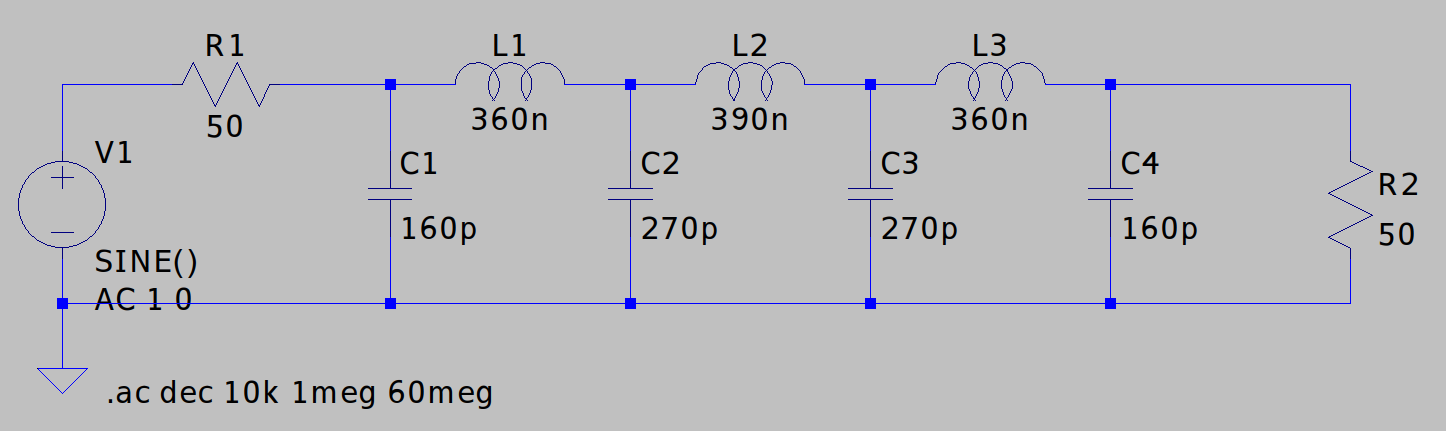
\includegraphics[width=\textwidth,keepaspectratio]{csebisev_390n_sch.png}}
		\label{fig:csebisev_390n_sch}
		\caption{Struktúra}
	\end{subfigure}
	\hfill
	\begin{subfigure}[b]{\textwidth}
		\centering
		\centerline{[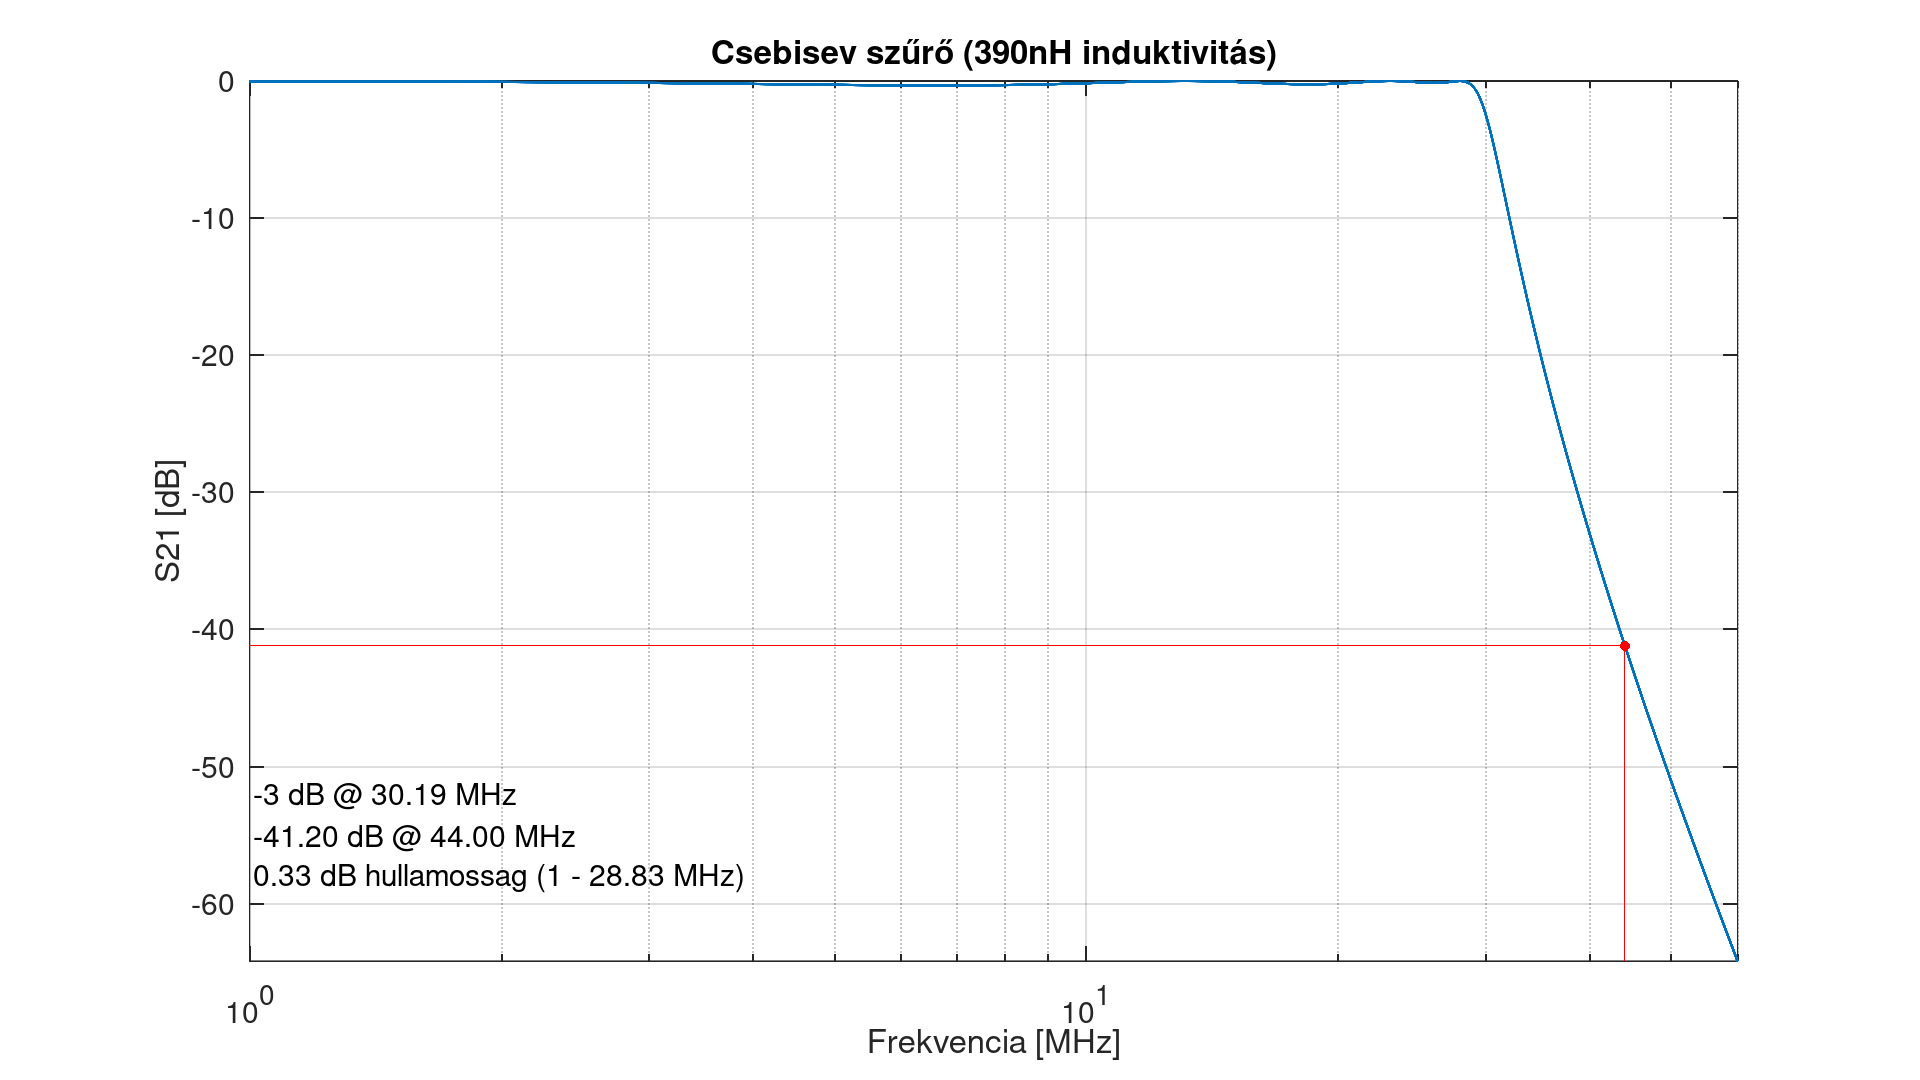
\includegraphics[width=1.3\textwidth,keepaspectratio]{csebisev_390n_bode.png}}
		\label{fig:csebisev_390n_bode}
		\caption{Frekvenciamenet}
	\end{subfigure}
	\caption{7-ed fokú Csebisev szűrő, 390nH induktivitással (E24-es sor)}
	\label{fig:csebisev_390n}
\end{figure}

\newpage


\subsection*{7-ed fokú Csebisev szűrő, kizárólag 360nH induktivitásokkal (E24-es sor)}

\begin{figure}[!ht]
	\centering
	\begin{subfigure}[b]{\textwidth}
		\centering
		\centerline{[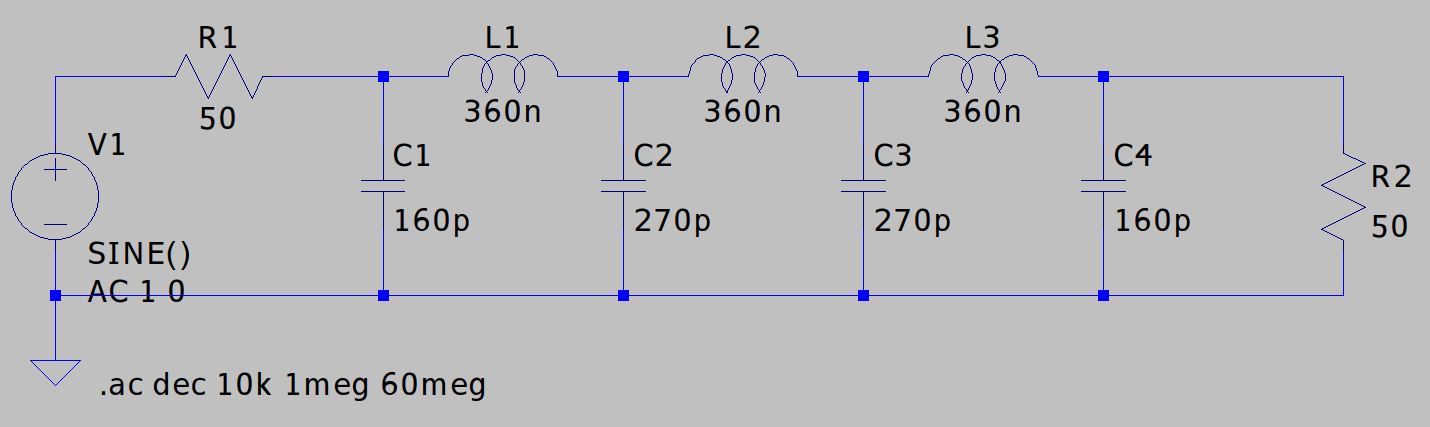
\includegraphics[width=\textwidth,keepaspectratio]{csebisev_360n_sch.png}}
		\label{fig:csebisev_360n_sch}
		\caption{Struktúra}
	\end{subfigure}
	\hfill
	\begin{subfigure}[b]{\textwidth}
		\centering
		\centerline{[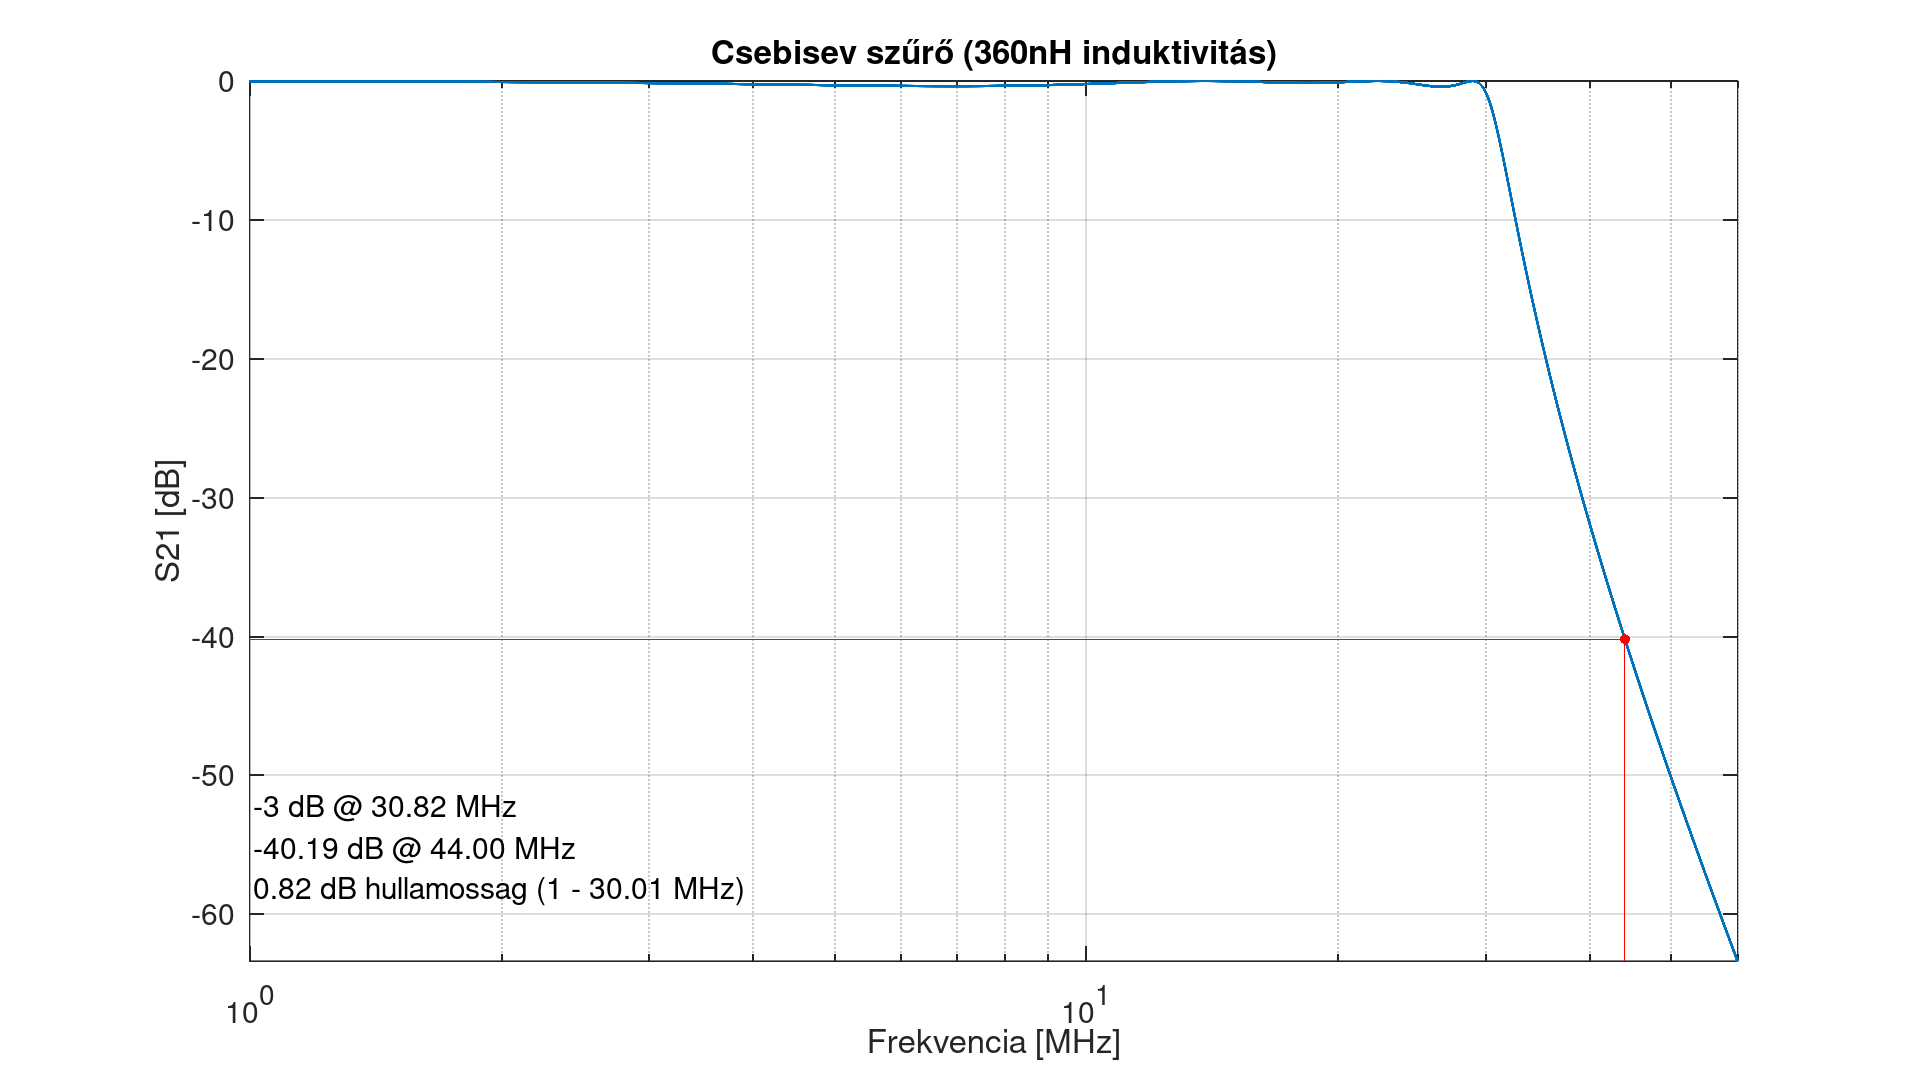
\includegraphics[width=1.3\textwidth,keepaspectratio]{csebisev_360n_bode.png}}
		\label{fig:csebisev_360n_bode}
		\caption{Frekvenciamenet}
	\end{subfigure}
	\caption{7-ed fokú Csebisev szűrő, kizárólag 360nH induktivitásokkal (E24-es sor)}
	\label{fig:csebisev_360n}
\end{figure}

\newpage


\subsection*{7-ed fokú Csebisev szűrő, 29,5\,MHz vágással és E12-es sorelemekkel}

\begin{figure}[!ht]
	\centering
	\begin{subfigure}[b]{\textwidth}
		\centering
		\centerline{[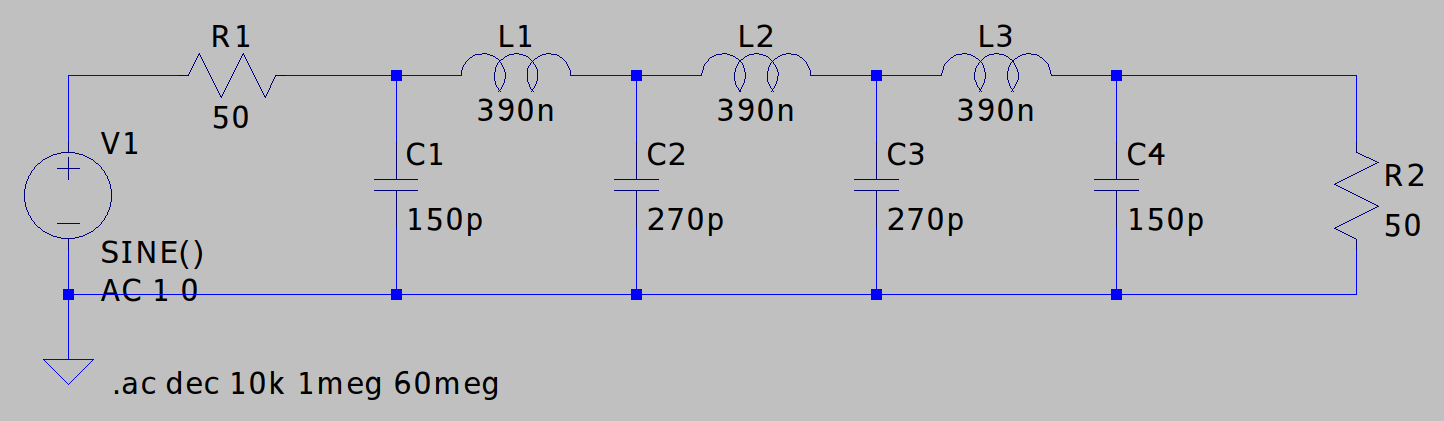
\includegraphics[width=\textwidth,keepaspectratio]{csebisev_295_sch.png}}
		\label{fig:csebisev_295_sch}
		\caption{Struktúra}
	\end{subfigure}
	\hfill
	\begin{subfigure}[b]{\textwidth}
		\centering
		\centerline{[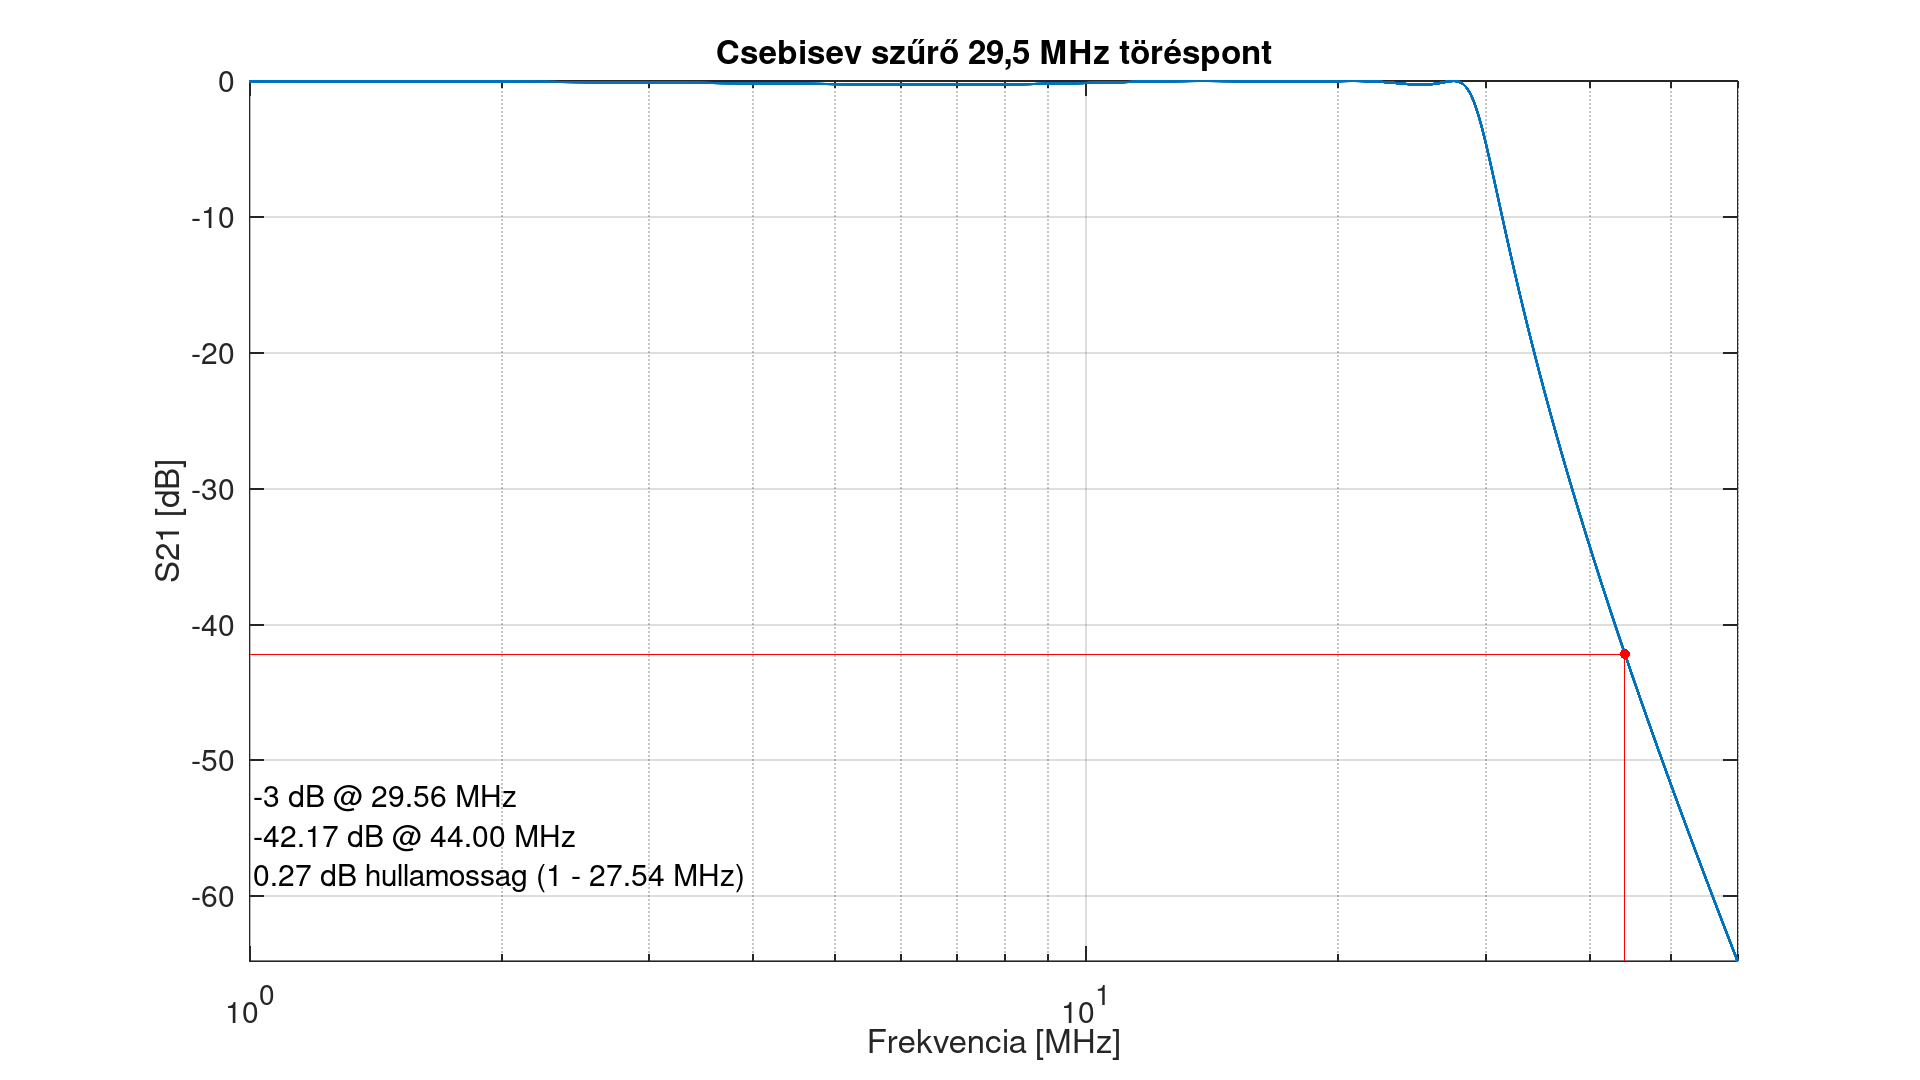
\includegraphics[width=1.3\textwidth,keepaspectratio]{csebisev_295_bode.png}}
		\label{fig:csebisev_295_bode}
		\caption{Frekvenciamenet}
	\end{subfigure}
	\caption{7-ed fokú Csebisev szűrő, 29,5\,MHz vágással és E12-es sorelemekkel}
	\label{fig:csebisev_295}
\end{figure}

\newpage

\end{document}